% each subsection is made of one or more frames
% frames are like slides
\subsection{Sub-Sección de Introducción} % CHANGE HERE THE SUBSECTION'S NAME
\label{subsec:intro} % ALSO CHANGE THE LABEL

% MAIN FRAME
% HERE YOU CAN PUT YOUR NAME, TITLE, AND A BRIEF DESCRIPTION OF YOUR THESIS
\begin{frame}
    \frametitle{Título del Frame}

    \centering
    \Large\textit{Título de la Tesis}
    % \Large\textit{Resolución neuro-simbólica del benchmark ARC-AGI usando LLMs ligeros y representación simbólica eficiente}

    \vspace{0.5cm}
    \textbf{Asesor}: Nombre del Asesor, Grado
    % \textbf{Asesor}: César Beltrán, PhD

    \vspace{0.8cm}
    \Large{Breve descripción del problema a resolver o de la propuesta de investigación.}
    % \Large{Proponer un \textbf{modelo ligero de IA} con \textbf{enfoque neuro-simbólico}, de modo que sirva para
    %     resolver problemas que involucren razonamiento abstracto de forma eficiente, tomando como referencia el
    %     \textbf{benchmark ARC-AGI} para su evaluación.}
\end{frame}

% here is an eaxmple of a timeline made with tikz
\begin{frame}
    \frametitle{Ejemplo de una Línea de Tiempo}

    \vspace{1cm}
    \begin{figure}[h!]
        \centering
        \scriptsize
        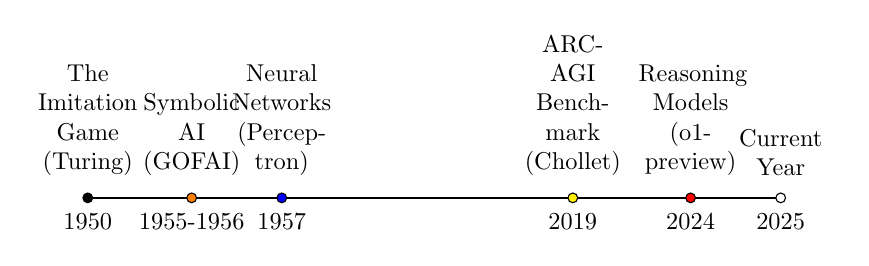
\begin{tikzpicture}[
                scale=0.88, transform shape
            ]
            % line
            \draw[thick] (0,0) -- (10,0);
            % nodes (x/date/label/color)
            \foreach \x/\date/\desc/\color in {
            0/1950/{The Imitation Game (Turing)}/black,
            1.5/1955-1956/{Symbolic AI (GOFAI)}/orange,
            2.8/1957/{Neural Networks (Perceptron)}/blue,
            7/2019/{ARC-AGI Benchmark (Chollet)}/yellow,
            8.7/2024/{Reasoning Models (o1-preview)}/red,
            10/2025/{Current Year}/white}
            {
            \draw[fill=\color] (\x,0) circle (2pt);
            \node[below=3pt] at (\x,0) {\date};
            \node[above, text width=1.5cm, align=center] at (\x,0.2) {\desc};
            }
        \end{tikzpicture}
        \vspace{0.8cm}
        \caption{Historia de la IA}
        \label{fig:timeline}
    \end{figure}

\end{frame}

\begin{frame}
    \frametitle{Ejemplo de una Imagen}

    El benchmark ARC-AGI fue propuesto por \cite{Cho19}.

    \vspace{0.3cm}
    \begin{figure}
        \centering
        \includegraphics[width=0.8\textwidth]{images/arc-agi}
        \vspace{0.2cm}
        \caption{Benchmark ARC-AGI}
        \label{fig:arc-agi}
    \end{figure}

\end{frame}

